\title[Causality]{Causality: Lecture 10}
\author[Joris Mooij]{\\[5mm]\large Joris Mooij \& Patrick Forr\'e\\
\url{j.m.mooij@uva.nl}, \url{p.d.forre@uva.nl}}
\institute[UvA]{University of Amsterdam}
\date[2022-04-12]{\normalsize April 12th, 2023}
\maketitle


\part{Equivalence Relations}
\frame{\partpage}

\begin{comment}
\begin{frame}{Equivalence relations}
Equivalence relations capture the notion that mathematical objects can be ``equivalent'' from some point of view.
\begin{Def}
  Let $Z$ be a set and $R \subseteq Z^2$ be a relation on $Z$ (i.e., a subset of ordered pairs of $Z$). $R$ is called an \emph{equivalence relation} if 
  \begin{enumerate}
    \item $R$ is reflexive: $(a,a) \in R$ for all $a \in Z$;
    \item $R$ is symmetric: $(a,b) \in R \iff (b,a) \in R$ for all $a,b \in Z$;
    \item $R$ is transitive: if $(a,b) \in R$ and $(b,c) \in R$ then $(a,c) \in R$ for all $a,b,c\in Z$.
  \end{enumerate}
\end{Def}
\end{frame}
\end{comment}

\begin{frame}{Equivalence of SCMs}
  \begin{Def}[\ref{def:equivalent_scms}]
  Let $M = \lt \Sin, \Send, \Srnd, \CX, P, f \rt$ and
  $\tilde{M} = \ltuple \Sin, \Send, \Srnd, \CX, P, \tilde{f} \rtuple$ be two SCMs.
  We say that
  $M$ is \emph{equivalent} to $\tilde{M}$ and write $M \equiv \tilde{M}$ if for each $v \in \Send$,
  $$\forall x \in \CX: \quad x_v = f_v(\xJ,\xV,\xW) \iff x_v = \tilde{f}_v(\xJ,\xV,\xW).$$
%  In words, $M$ and $\tilde{M}$ are considered equivalent if they at most differ in terms of their
%  causal mechanisms, yet each of their structural equations has the same solutions.
\end{Def}
\begin{Prp}[\ref{prp:equivalent_scms}]
\begin{enumerate}
  \item Equivalence of SCMs is preserved by hard interventions.
  \item Unique solvability is invariant under SCM equivalence.
  \item Simplicity is invariant under SCM equivalence.
  \item Equivalent SCMs have the same solution functions, solutions, (potential) outcomes, and Markov kernels.
\end{enumerate}
\end{Prp}
\end{frame}

\begin{frame}{Example}
\begin{Eg}
  Is the SCM with the single structural equation
  $$X = -X^3 + X + W$$
  where $X$ is endogenous, and $W$ is exogenous, equivalent to the SCM obtained by replacing the structural equation with
  $$X = \sqrt[3]{W}$$
  (note that $X$ no longer appears on the r.h.s.)?

  \bigskip
  \uncover<2- |handout:0>{Yes, it is!}
\end{Eg}
\end{frame}

\begin{frame}{Example}
\begin{Eg}
  Is the SCM with endogenous variable $X \in \RN$ and exogenous random variable $W \in \RN$ and structural equation
  $$X = W X + c$$
  equivalent to the SCM obtained by replacing the structural equation with
  $$X = \begin{cases}
          \xi & W = 1 \\
          \frac{c}{1 - W} & W \ne 1
        \end{cases}$$
  for some choice of $\xi \in \RN$ and $P(W)$?

  \bigskip
  \uncover<2- |handout:0>{No, it is not! No matter how we choose $\xi$, and not even when $P(W=1) = 0$.}
\end{Eg}
  \uncover<2- |handout:0>{If one does not model interventions on exogenous random variables (like e.g.\ Pearl), weaker notions of equivalence can be used (see \cite{BFPM21}).}
\end{frame}

\begin{frame}{Other equivalences: definition}
  \begin{Def}[\ref{def:scm_obs_interv_equiv}]
  Let $M = \lt \Sin, \Send, \Srnd, \CX, P, f \rt$ and
  $\tilde{M} = \ltuple \tilde{\Sin}, \tilde{\Send}, \tilde{\Srnd}, \tilde{\CX}, \tilde{P}, \tilde{f} \rtuple$ be two simple SCMs
  and $O \subseteq (\Send \cap \tilde{\Send}) \cup (\Srnd \cap \tilde{\Srnd})$ a common subset.
  We say that:
  \begin{enumerate}
    \item $M$ and $\tilde{M}$ are \emph{observably equivalent w.r.t.\ $O$} if $\CX_O = \tilde{\CX}_O$, $\CX_{J \cap \tilde{J}} = \tilde{\CX}_{J \cap \tilde{J}}$ and their marginal Markov kernels coincide:
      $$P_{M}(X_O \mid \doit(X_J)) = P_{\tilde{M}}(X_O \mid \doit(X_{\tilde J})).$$
    This has to be interpreted as both Markov kernels being a version of a Markov kernel $\CX_{J \cap \tilde{J}} \dshto \CX_O$,
    i.e., $P_{M}(X_O \mid \doit(X_J))$ must be essentially constant in $x_{J \setminus \tilde{J}}$ and
    $P_{\tilde{M}}(X_O \mid \doit(X_{\tilde{J}}))$ must be essentially constant in $x_{\tilde{J} \setminus J}$;
%    \item $M$ and $\tilde{M}$ are \emph{observably equivalent w.r.t.\ $O$} if $\CX_O = \tilde{\CX}_O$, $J = \tilde{J}$, $\CX_J = \tilde{\CX}_J$ and $P_{M}(X_O \mid \doit(\XJ)) = P_{\tilde{M}}(X_O \mid \doit(\XJ))$;
    \item $M$ and $\tilde{M}$ are \emph{interventionally equivalent w.r.t.\ $O$} if for every subset $T \subseteq O$ the intervened SCMs $M_{\doit(T)}$ and $\tilde{M}_{\doit(T)}$ are observably equivalent w.r.t.\ $O \setminus T$.
%    \item $M$ and $\tilde{M}$ are said to be \emph{counterfactually equivalent w.r.t.\ $O$} if the twin SCMs $M^\twin$ and $\tilde{M}^\twin$ are interventionally equivalent w.r.t.\ $O \cup O'$, where $O'$ is the copy of $O$ in $\Send' \cap \tilde{\Send}'$.
  \end{enumerate}
\end{Def}
\end{frame}

\begin{frame}{Other equivalences: relationships}
  \begin{Prp}[\ref{prp:pearls_ladder_levels_1_and_2}]
  For simple SCMs $M, \tilde{M}$ and a subset $O \subseteq (\Send \cap \tilde{\Send}) \cup (\Srnd \cap \tilde{\Srnd})$:
  \begin{enumerate}
%    \item If $M \equiv \tilde{M}$ then $M$ and $\tilde{M}$ are counterfactually equivalent w.r.t.\ $O$.
    \item If $M$ and $\tilde{M}$ are equivalent, then 
      $M$ and $\tilde{M}$ are interventionally equivalent w.r.t.\ $O$.
    \item If $M$ and $\tilde{M}$ are interventionally equivalent w.r.t.\ $O$ then 
      $M$ and $\tilde{M}$ are observably equivalent w.r.t.\ $O$.
  \end{enumerate}
\end{Prp}
The reverse implications do not hold in general. This expresses that causal modeling is more refined than probabilistic modeling.
\end{frame}

\begin{frame}{Example}
\begin{Eg}
  The following SCMs are both simple:
  \begin{align*}
    M &: \qquad N \sim \C{N}(\mu,\sigma^2) \qquad C = \alpha + \beta N \\
    \tilde{M}&: \qquad C \sim \C{N}(\tilde{\mu},\tilde{\sigma}^2) \qquad N = \tilde{\alpha} + \tilde{\beta} C
  \end{align*}
Their distributions are respectively 
  $$P_M\left(\begin{pmatrix}N \\C\end{pmatrix}\right) = \C{N}\left(\begin{pmatrix} \mu \\ \alpha + \beta \mu \end{pmatrix}, \begin{pmatrix} \sigma^2 & \beta\sigma^2 \\ \beta\sigma^2 & \beta^2\sigma^2\end{pmatrix}\right)$$
and
  $$P_{\tilde{M}}\left(\begin{pmatrix}N\\C\end{pmatrix}\right) = \C{N}\left(\begin{pmatrix} \tilde{\alpha} + \tilde{\beta}\tilde{\mu} \\ \tilde{\mu} \end{pmatrix}, \begin{pmatrix} \tilde{\beta}^2\tilde{\sigma}^2 & \tilde{\beta}\tilde{\sigma}^2 \\ \tilde{\beta}\tilde{\sigma}^2 & \tilde{\sigma}^2\end{pmatrix}\right)$$
For which parameters are they observably equivalent (w.r.t.\ $N,C$)?
For which parameters are they interventionally equivalent (w.r.t.\ $N,C$)?
\end{Eg}
\end{frame}

\part{Marginalizations}
\frame{\partpage}

\begin{frame}{Marginalizations: Motivation}
  Often we like to obtain a simpler description of a system by hiding irrelevant details of a subsystem.

  \begin{Eg}
    \begin{enumerate}
      \item Moving code into a subroutine when programming
      \item Marginalizing a probability distribution over some variables
      \item Taking an orthogonal projection in linear algebra
      \item Taking a latent projection of a CDMG
    \end{enumerate}
  \end{Eg}

  For SCMs, we define a marginalization over a subset of endogenous variables that removes those
  variables from the model but preserves the causal semantics of the remaining variables.
\end{frame}

\begin{frame}{Marginalizations: Basic insight}
  Write $K := V \setminus L$ and let $\tilde{g}_L$ denote the unique solution function of $M_{[L]}$.
    \begin{equation*}\begin{split}
%  & \begin{cases}
%    x_L = g_L(x_J,x_W) \\
%    x_M = g_M(x_J,x_W) \\
%  \end{cases} \\
%  \iff 
  & \begin{cases}
    x_L = f_L(x_J,x_K,x_L,x_W) \\
    x_K = f_K(x_J,x_K,x_L,x_W) \\
  \end{cases} \\
  \iff & \begin{cases}
    x_L = \tilde{g}_L(x_J,x_K,x_W) \\
    x_K = f_K(x_J,x_K,x_L,x_W) \\
  \end{cases}  \\
  \iff & \begin{cases}
    x_L = \tilde{g}_L(x_J,x_K,x_W) \\
    x_K = f_K(x_J,x_K,\tilde{g}_L(x_J,x_K,x_W),x_W) =: \tilde{f}(\xJ,x_{K},\xW) \\
  \end{cases} \\
%  \iff & \begin{cases}
%    x_L = \tilde{g}_L(x_J,x_K,x_W) \\
%    x_K = \tilde{f}(x_J,x_K,x_W) \\
%  \end{cases}
  \end{split}\end{equation*}
  We can now forget $x_L$, and only retain:
  $$x_K = \tilde{f}(x_J,x_K,x_W)$$
\end{frame}

\begin{frame}{Marginalizations: Definition}
  \begin{Def}[\ref{def:scm_marginalization}]
  Let $M = \lt \Sin, \Send, \Srnd, \CX, P, f \rt$ be an SCM and $L \subseteq \Send$ such that
  the submodel $M_{[L]}$ is uniquely solvable.
  Let $\tilde{g}_L : \CX_{\Sin} \times \CX_{V \sm L} \times \CXW \to \CX_L$
  be the unique solution function for $M_{[L]}$.
  Then we call $M_{\setminus L} = \ltuple \Sin, V \sm L, \Srnd, \CX_{\Sin} \times \CX_{V \sm L} \times \CX_{\Srnd}, P, \tilde{f} \rtuple$ with
  $$\tilde{f}(\xJ,x_{V \sm L},\xW) = f_{V \sm L}(\xJ,x_{V \sm L},\tilde{g}_L(\xJ,x_{V \sm L},\xW),\xW)$$
  the \emph{marginalization of $M$ over $L$}.
\end{Def}
The marginalization is obtained by performing the following steps:
  \begin{enumerate}
    \item Solve the submodel $M_{[L]}$ on $L$
    \item Substitute the solution function into the causal mechanism for $V \sm L$
    \item Restrict to the $V \sm L$ component only
  \end{enumerate}
\end{frame}

\begin{frame}{Marginalization: Properties I}
  \begin{Lem}[\ref{lem:marginalization_preserves_unique_solvability}]
  Let $M$ be an SCM such $M_{[L]}$ is uniquely solvable for $L \subseteq \Send$.
  If $M$ is uniquely solvable then 
  \begin{itemize}
    \item its marginalization $M_{\setminus L}$ is uniquely solvable; 
    \item the unique solution function for $M_{\setminus L}$ is $g_{V\setminus L}$, where 
  $g : \CX_J \times \CX_W \to \CX_V$ is the unique solution function for $M$.
  \end{itemize}
\end{Lem}

This gives:
$$P_{M_{\setminus L}}(X_{V\setminus L},X_W \mid \doit(X_J)) = P_{M}(X_{V\setminus L},X_W \mid \doit(X_J))$$
(The Markov kernel of the marginalized SCM is given by the marginal Markov kernel of the SCM).
This explains the name `marginalization'.
\end{frame}
  
\begin{frame}{Marginalization: Properties II}
  \begin{Prp}[\ref{prp:interventions_marginalizations_commute}]
    Let $M$ be an SCM such $M_{[L]}$ is uniquely solvable for $L \subseteq \Send$.
    For a hard intervention $\doit(T\dots)$ with target $T \subseteq \Sin \cup \Srnd \cup \Send$ (of any of the three variants) such that $L \cap T = \emptyset$:
    $$(M_{\doit(T\dots)})_{\setminus L} = (M_{\setminus L})_{\doit(T\dots)}.$$
\end{Prp}
Try proving this yourself!

\begin{Prp}[\ref{prp:marginalization_commutes}]
  Let $M$ be an SCM and $L_1, L_2 \subseteq \Send$ such that $L_1 \cap L_2 = \emptyset$.
  If $M_{[L_1]}$ and $(M_{\setminus L_1})_{[L_2]}$ are uniquely solvable, then $M_{[L_1\cup L_2]}$ is uniquely solvable, and:
  $$(M_{\setminus L_1})_{\setminus L_2} = M_{\setminus (L_1\cup L_2)}.$$
\end{Prp}
\begin{proof}
  Straightforward, but cumbersome notation. See lecture notes.
\end{proof}
\end{frame}

\begin{frame}{Marginalization: Properties for Simple  SCMs}
Let $M = \lt \Sin, \Send, \Srnd, \CX, P, f \rt$ be a simple SCM.
\begin{Prp}[\ref{prp:marginalization_preserves_simplicity}]
  For any $L \subseteq \Send$, the marginalization $M_{\setminus L}$ is also simple.
\end{Prp}
\begin{proof}
  \uncover<2- |handout:0>{%
  For $T \subseteq J \cup W \cup V \setminus L$, marginalization commutes with hard intervention:
  $$(M_{\setminus L})_{\doit(T)} = (M_{\doit(T)})_{\setminus L}.$$
  Because $M$ is simple, also $M_{\doit(T)}$ is simple, and in particular it is
  uniquely solvable. 
  Hence its marginalization $(M_{\doit(T)})_{\setminus L}$ is uniquely solvable.
  This means that $(M_{\setminus L})_{\doit(T)}$ is uniquely solvable. Since this
  holds for any $T$, $M_{\setminus L}$ is simple.
  }
\end{proof}
\begin{Cor}[\ref{cor:marginalization_commutes_simple_scm}]
  For $L_1, L_2 \subseteq \Send$ with $L_1 \cap L_2 = \emptyset$:
    $(M_{\setminus L_1})_{\setminus L_2} = (M_{\setminus L_2})_{\setminus L_1} = M_{\setminus (L_1 \cup L_2)}$.
\end{Cor}
\end{frame}

\begin{frame}{Marginalizations preserve causal semantics}
\begin{Thm}[\ref{thm:various_equiv_marginalization}]
  Let $M = \lt \Sin, \Send, \Srnd, \CX, P, f \rt$ be a simple SCM and $L \subseteq \Send$.
  Then $M$ and $M_{\setminus L}$ are observably and
  interventionally %and counterfactually 
  equivalent w.r.t.\ $(V \cup W) \setminus L$.
\end{Thm}
\begin{proof}
  \uncover<2- |handout:0>{%
  Write $K := V \setminus L$. We already noticed that
  $P_{M}(X_K,X_W \mid \doit(X_J)) = P_{M_{\setminus L}}(X_K,X_W \mid \doit(X_J))$.

  Let $T \subseteq K \cup W$. Then $(M_{\setminus L})_{\doit(T)} = (M_{\doit(T)})_{\setminus L}$.
  The observable equivalence of $M_{\doit(T)}$ and $(M_{\doit(T)})_{\setminus L}$ w.r.t.\ $(K \cup W) \setminus T$ hence implies the observable equivalence of $M_{\doit(T)}$ and $(M_{\setminus L})_{\doit(T)}$ w.r.t.\ $(K \cup W) \setminus T$.
  Hence, $M$ and $M_{\setminus L}$ are interventionally equivalent w.r.t.\ $K \cup W$.}
\end{proof}
Note: this can be shown for general (non-simple) SCMs as well.
\end{frame}

\begin{comment}
\begin{frame}{Linear SCMs}
  \begin{Def}
We call an SCM $M=\lt \Sin, \Send, \Srnd, \CX, P, f \rt$
\emph{linear} if all variables are real-valued and
each component of the causal mechanism is an affine combination of endogenous variables, that is
$$
%  f_v(x) = \sum_{w\in V \cup J \cup W} B_{vw} x_w,
    f_v(x) = \sum_{u\in V} B_{vu}(x_J,x_W) x_u + c_v(x_J,x_W),
$$
    where $B(x_J,x_W)\in\RN^{V \times V}$ is a matrix-valued function $\CXJ\times\CXW \to \RN^{V\times V}$ and
$c(x_J,x_W) \in \RN^V$ is a vector-valued function $\CXJ\times\CXW \to \RN^V$.
  \end{Def}

  \begin{Prp}
Let $L \subseteq V$.
$(M)_{\doit(V\setminus L)}$ is uniquely solvable if and only if 
$I_{L}-B_{LL}(x_J,x_W)$ are invertible $\forall x_J \in \CX_J, x_W \in \CX_W$,
with unique solution function:
\small
  \begin{equation*}\begin{split}
    g &: \RN^{V\setminus L} \times \RN^{J\cup W} \to \RN^L \\
      &: (x_{V\setminus L},x_J,x_W) \mapsto (I_L - B_{LL}(x_J,x_W))^{-1} \big(B_{L,{V\setminus L}}(x_J,x_W) x_{V\setminus L} + c_{L}(x_J,x_W)\big).
  \end{split}\end{equation*}
  \end{Prp}
\end{frame}
\end{comment}

\part{Graphs}
\frame{\partpage}

\begin{frame}{Finally, graphs!}
  We introduce the graph of an SCM with nodes corresponding to the variables and directed edges representing the functional relationships, i.e., the structure of the structural equations.
  
  \begin{Def}[\ref{def:scm_parent}]
  For $i \in \Sin \cup \Send \cup \Srnd$ and $j \in \Send$, we say that
  \emph{$i$ is a parent of $j$ according to $M$} if there does not exist a measurable function
  $\tilde f_j : \CX_{(\Sin\cup\Send\cup\Srnd) \setminus \{i\}} \to \CX_j$
  such that for all $x \in \CX$,
  $$x_j = f_j(x) \iff x_j = \tilde f_j(x_{\setminus i}),$$
  where $x_{\setminus i}$ is shorthand for $x_{(\Sin\cup\Send\cup\Srnd)\setminus\{i\}}$.
\end{Def}
  \begin{itemize}
    \item In words: $i$ is parent of $j$ if the causal mechanism for $j$ is not equivalent to one that is constant w.r.t.\ its input component $i$.
    \item By definition, exogenous (input and random) variables have no parents.
    \item Note that the parent-relationship is preserved under equivalence.
  \end{itemize}
\end{frame}

\begin{frame}{Graphs: Definition}
  \begin{Def}[\ref{def:scm_graph}]
  The CDG $\lt \Sin, \Send \cup \Srnd, E \rt$ with
  input nodes $\Sin$, output nodes $\Send\cup\Srnd$, and
  directed edges
  $$E = \{i \to j : i \in \Sin\cup\Srnd\cup\Send, j\in\Send: \text{$i$ is parent of $j$ according to $M$}\}$$
  is called the \emph{graph of the SCM $M$} and will be denoted as $G(M)$.
\end{Def}
  \begin{itemize}
    \item Equivalent SCMs have the same graphs.
    \item Observably equivalent SCMs may have different graphs.
    \item Interventionally equivalent SCMs may have different graphs.
  \end{itemize}
\end{frame}

\begin{frame}{Example}
  \begin{Eg}
    \begin{itemize}
      \item Consider an SCM $M$
  with endogenous variables $X,Y$ and exogenous random variable $W$ and structural equations
    $$X = -X^3 + X + W, \qquad Y = \sin(X) - W$$
  \item Its graph is $G(M)$: \\
  \centerline{\begin{tikzpicture}
    \node[var] (W) at (0,0) {$W$};
    \node[var] (X) at (1.5,0) {$X$};
    \node[var] (Y) at (3,0) {$Y$};
    \uncover<2- |handout:0>{
    \draw[arr] (W) -- (X);
    \draw[arr,bend left] (W) edge (Y);
    \draw[arr] (X) -- (Y);}
  \end{tikzpicture}}
\item Note: $X$ is not a parent of itself, because
  its structural equation is equivalent to $X = \sqrt[3]{W},$
  where $X$ does not appear on the r.h.s..
\item
  When considering exogenous random variables as latent, we can consider the marginalized graph $G(M)^{\setminus W}$:\\

  \medskip
  \centerline{\begin{tikzpicture}
    \node[var] (X) at (1.5,0) {$X$};
    \node[var] (Y) at (3,0) {$Y$};
    \uncover<2- |handout:0>{
    \draw[biarr,bend left] (X) edge (Y);
    \draw[arr] (X) -- (Y);
  }
  \end{tikzpicture}}
    \end{itemize}
  \end{Eg}
\end{frame}

\begin{frame}{Example: Self-cycle}
\begin{Eg}
  The graph of an SCM with structural equation
  $$X = W X + c$$
  ($X$ endogenous, $W$ exogenous random) has a \emph{self-cycle} at $X$:\\
  \centerline{\begin{tikzpicture}
    \node[var] (W) at (0,0) {$W$};
    \node[var] (X) at (1.5,0) {$X$};
    \draw[arr] (W) -- (X);
    \draw[arr,in=30,out=-30,looseness=5] (X) edge (X);
  \end{tikzpicture}}
\end{Eg}
Self-cycles are a warning sign of complications with respect to solvability.
They are of no concern when restricting to the class of simple SCMs.
  \begin{Prp}[\ref{prp:self-cycles}]
  For $j \in V$, we have that there is a self-cycle $j \to j$ in $G(M)$ if and only if
  $M_{[j]}$ is \emph{not} uniquely solvable.
  In particular, graphs of simple SCMs have no self-cycles.
\end{Prp}
\end{frame}

\begin{frame}{Compatibility of operations on SCMs and graphs}
  \begin{Prp}[\ref{prp:compatibility_graph}]
  \begin{itemize}
    \item Hard interventions: for $T \subseteq J \cup V \cup W$,
      $$G(M_{\doit(T)}) = G(M)_{\doit(T)}.$$
    \item Marginalizations: If $M$ is simple, then for $L \subseteq V$,
      $$G(M_{\setminus L}) \subseteq G(M)^{\setminus L}.$$
  \end{itemize}
\end{Prp}
\begin{proof}
Try proving the first statement yourself!
The second statement is more involved. For a proof by induction, see the lecture notes.
\end{proof}
\end{frame}

\part{Acyclic SCMs}
\frame{\partpage}

\begin{frame}{Acyclic SCMs}
  \begin{Def}[\ref{def:scm_acyclic}]
  An SCM $M$ is called \emph{acyclic} if its graph $G(M)$ is acyclic.
\end{Def}
  While most literature only considers acyclic SCMs (or CBNs), we propose to
  use simple SCMs instead if one cannot rule out a priori the possibility of causal cycles.
  \begin{Prp}[\ref{prp:acyclic_scms_are_simple}]
  Acyclic SCMs are simple.
\end{Prp}
\begin{proof}
  Main idea: Choose a topological ordering and solve the system of structural equations in that order.
  For details, see lecture notes.
\end{proof}
\end{frame}

\begin{frame}{Relations between causal models}
  \centerline{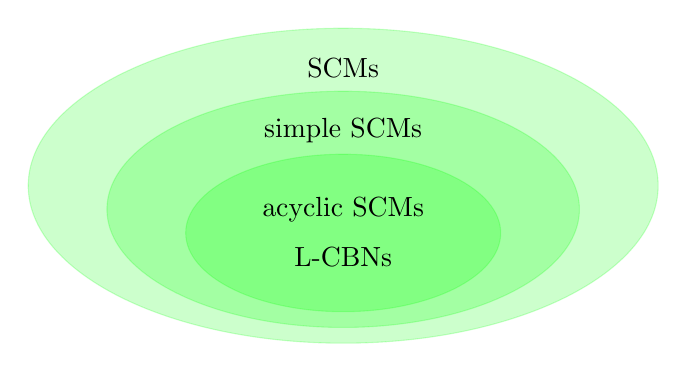
\begin{tikzpicture}
      \begin{scope}
%        \draw[draw=green,fill=green,opacity=0.2] (0,0) ellipse (1.5cm and 0.5cm);
        \draw[draw=green,fill=green,opacity=0.2] (0,0.3) ellipse (2cm and 1cm);
        \draw[draw=green,fill=green,opacity=0.2] (0,0.6) ellipse (3cm and 1.5cm);
        \draw[draw=green,fill=green,opacity=0.2] (0,0.9) ellipse (4cm and 2cm);
        \node at (0,0) {L-CBNs};
        \node at (0,0.6) {acyclic SCMs};
        \node at (0,1.6) {simple SCMs};
        \node at (0,2.4) {SCMs};
      \end{scope}
  \end{tikzpicture}}

  \bigskip
  \begin{itemize}
    \item L-CBNs are interventionally equivalent to acyclic SCMs.
    \item Simple SCMs are more expressive than acyclic SCMs (or L-CBNs), because they
  can model causal cycles due to weak feedback loops.
  \item SCMs are even more expressive, but also much more complicated to work with.
  \end{itemize}
\end{frame}

\begin{frame}{Interventional equivalence of acyclic SCMs and L-CBNs}
  \begin{Def}[Informal version of \ref{def:interventional_equivalence_cbn_scm}]
    An SCM and an L-CBN are interventionally equivalent w.r.t.\ a subset of variables if all their intervened Markov kernels have the same marginal on this subset.
  \end{Def}
  \begin{Prp}[\ref{prp:interventional_equivalence_cbn_scm}]
  \begin{enumerate}
%    \item Given an acyclic SCM $M$, we can construct a CBN $\tilde{M}$ that is interventionally equivalent to it (w.r.t.\ $O = V \cup W$).
    \item Given an acyclic SCM $M$ with endogenous variables $V$, endogenous variables $W$ and an observed subset $O \subseteq V \cup W$, we can construct an L-CBN $\tilde{M}$ with observed output variables $O$ and graph $G(M)$ that is interventionally equivalent to $M$ w.r.t.\ $O$.
    \item Given an L-CBN $\tilde{M}$ with graph $G^+$ and observed output variables $O$, we can construct an acyclic SCM $M$ with marginal graph $G^+$ that is interventionally equivalent to $\tilde{M}$ w.r.t.\ $O$.
  \end{enumerate}
  \end{Prp}
\end{frame}

\part{Cyclic SCMs}
\frame{\partpage}

\begin{frame}{Modeling feedback loops}
  \begin{itemize}
    \item Feedback loops are often present in systems;
    \item Such systems are usually described as a system of (random) differential equations;
  \end{itemize}

  \bigskip
The \emph{equilibrium} states of such systems can sometimes be causally modelled by a (cyclic) SCM.

\bigskip
We consider two examples:
  \begin{enumerate}
    \item Damped coupled harmonic oscillator (simple SCM)
    \item Price-supply-demand (non-simple SCM)
  \end{enumerate}
and prove that cyclic SCMs are simple if the causal mechanisms are sufficiently weak and smooth.
\end{frame}

\begin{frame}{Example I: Damped Coupled Harmonic Oscillator}
  \centerline{\scalebox{0.8}{\begin{tikzpicture}
    \begin{scope}
      \fill[pattern=north east lines,draw=none] (-1,-1) rectangle (0,1);
      \draw (0,-1) -- (0,1);
      \begin{scope}[yshift=5mm]
      \node (Q1) at (2,0) {$m_1$};
      \node (Q2) at (4,0) {$m_2$};
      \node (Q3) at (6,0) {$m_3$};
      \node (Q4) at (8,0) {$m_4$};
      \node (Q5) at (10,0) {$m_5$};
      \end{scope}
      \begin{scope}[yshift=-5mm]
        \node (l0) at (1,0) {$\ell_0$};
        \node (l1) at (3,0) {$\ell_1$};
        \node (l2) at (5,0) {$\ell_2$};
        \node (l3) at (7,0) {$\ell_3$};
        \node (l4) at (9,0) {$\ell_4$};
        \node (l5) at (11,0) {$\ell_5$};
      \end{scope}
      \fill[black] (2,0) circle (.2);
      \fill[black] (4,0) circle (.2);
      \fill[black] (6,0) circle (.2);
      \fill[black] (8,0) circle (.2);
      \fill[black] (10,0) circle (.2);
      \draw (12,-1) -- (12,1);
      \fill[pattern=north east lines,draw=none] (12,-1) rectangle (13,1);
      \draw[thick,decorate,decoration={coil,aspect=0.7,amplitude=4,segment length=3mm}] (0,0) -- (2,0);
      \draw[thick,decorate,decoration={coil,aspect=0.7,amplitude=4,segment length=3mm}] (2,0) -- (4,0);
      \draw[thick,decorate,decoration={coil,aspect=0.7,amplitude=4,segment length=3mm}] (4,0) -- (6,0);
      \draw[thick,decorate,decoration={coil,aspect=0.7,amplitude=4,segment length=3mm}] (6,0) -- (8,0);
      \draw[thick,decorate,decoration={coil,aspect=0.7,amplitude=4,segment length=3mm}] (8,0) -- (10,0);
      \draw[thick,decorate,decoration={coil,aspect=0.7,amplitude=4,segment length=3mm}] (10,0) -- (12,0);
      \node at (0,1.3) {\tiny $Q_0$};
      \node at (12,1.3) {\tiny $Q_6$};
    \end{scope}
  \end{tikzpicture}}}

Dynamics:
$$ \frac{d^2Q_i}{dt^2} = \frac{k_i}{m_i} (Q_{i+1} - Q_i - \ell_i) + \frac{k_{i-1}}{m_i} (Q_{i-1} - Q_i + \ell_{i-1}) -\frac{b_i}{m_i} \frac{dQ_i}{dt} \qquad i=1,\dots,d.  $$
At equilibrium (set $\frac{d^2Q_i}{dt^2} = \frac{d Q_i}{dt} = 0$ and solve each equation for $Q_i$):
$$Q_i = \frac{k_i(Q_{i+1} - \ell_i) + k_{i-1}(Q_{i-1}+\ell_{i-1})}{k_i + k_{i-1}} \qquad i=1,\dots,d.$$

  \centerline{\scalebox{0.8}{\begin{tikzpicture}
    \begin{scope}[yshift=-3cm]
      \node[varc] (Q0) at (0,0) {$Q_0$};
      \node[var] (Q1) at (2,0) {$Q_1$};
      \node[var] (Q2) at (4,0) {$Q_2$};
      \node[var] (Q3) at (6,0) {$Q_3$};
      \node[var] (Q4) at (8,0) {$Q_4$};
      \node[var] (Q5) at (10,0) {$Q_5$};
      \node[varc] (Q6) at (12,0) {$Q_6$};
      \node[varc] (K0) at (1,1) {$k_0$};
      \node[varc] (K1) at (3,1) {$k_1$};
      \node[varc] (K2) at (5,1) {$k_2$};
      \node[varc] (K3) at (7,1) {$k_3$};
      \node[varc] (K4) at (9,1) {$k_4$};
      \node[varc] (K5) at (11,1) {$k_5$};
      \node[varc] (L0) at (1,-1) {$\ell_0$};
      \node[varc] (L1) at (3,-1) {$\ell_1$};
      \node[varc] (L2) at (5,-1) {$\ell_2$};
      \node[varc] (L3) at (7,-1) {$\ell_3$};
      \node[varc] (L4) at (9,-1) {$\ell_4$};
      \node[varc] (L5) at (11,-1) {$\ell_5$};
      \draw[arr] (Q0) to (Q1);
      \draw[arr,bend left=20] (Q1) to (Q2);
      \draw[arr,bend left=20] (Q2) to (Q3);
      \draw[arr,bend left=20] (Q3) to (Q4);
      \draw[arr,bend left=20] (Q4) to (Q5);
      \draw[arr,bend left=20] (Q5) to (Q4);
      \draw[arr,bend left=20] (Q4) to (Q3);
      \draw[arr,bend left=20] (Q3) to (Q2);
      \draw[arr,bend left=20] (Q2) to (Q1);
      \draw[arr] (Q6) to (Q5);
      \draw[arr] (K0) -- (Q1);
      \draw[arr] (K1) -- (Q1);
      \draw[arr] (K1) -- (Q2);
      \draw[arr] (K2) -- (Q2);
      \draw[arr] (K2) -- (Q3);
      \draw[arr] (K3) -- (Q3);
      \draw[arr] (K3) -- (Q4);
      \draw[arr] (K4) -- (Q4);
      \draw[arr] (K4) -- (Q5);
      \draw[arr] (K5) -- (Q5);
      \draw[arr] (L0) -- (Q1);
      \draw[arr] (L1) -- (Q1);
      \draw[arr] (L1) -- (Q2);
      \draw[arr] (L2) -- (Q2);
      \draw[arr] (L2) -- (Q3);
      \draw[arr] (L3) -- (Q3);
      \draw[arr] (L3) -- (Q4);
      \draw[arr] (L4) -- (Q4);
      \draw[arr] (L4) -- (Q5);
      \draw[arr] (L5) -- (Q5);
  \end{scope}
  \end{tikzpicture}}}
\end{frame}

\begin{frame}{Example II: Price, supply and demand}
  \begin{topalignedcolumn}{0.65\linewidth}
  \begin{description}
     \item[$D$] demand of a quantity of a product
     \item[$S$] supply of a quantity of a product
     \item[$R$] price of the product
  \end{description}
  \end{topalignedcolumn}\hfill%
  \begin{topalignedcolumn}{0.3\linewidth}
    \scalebox{0.8}{\begin{tikzpicture}
%      \node at (-2.5,2) {(c)};
    \node[var] (ED) at (1.5,0) {$E_D$};
    \node[var] (D) at (1.5,-1) {$D$};
    \node[var] (ES) at (-1.5,0) {$E_S$};
    \node[var] (S) at (-1.5,-1) {$S$};
    \node[var] (P) at (0,-1) {$R$};
    \draw[arr, bend left=20] (P) edge (S);
    \draw[arr, bend left=20] (P) edge (D);
    \draw[arr, bend left=20] (S) edge (P);
    \draw[arr, bend left=20] (D) edge (P);
    \draw[arr] (ED) to (D);
    \draw[arr] (ES) to (S);
    \draw[arr] (P)  to [out=62,in=118,looseness=4.4] (P);
    \end{tikzpicture}}
  \end{topalignedcolumn}

  \medskip
  Market dynamics:
$$\begin{aligned}
    D &= \beta_D R + E_D \\
    S &= \beta_S R + E_S \\
    \frac{dR}{dt} &= D - S,
  \end{aligned}$$
  At market equilibrium ($\frac{dR}{dt}=0$) we get an SCM with causal mechanism:
$$
  \begin{aligned}
    f_D(d,s,r,e_D,e_S) &:= \beta_D r + e_D \\
    f_S(d,s,r,e_D,e_S) &:= \beta_S r + e_S \\
    f_P(d,s,r,e_D,e_S) &:= r + (d - s).
  \end{aligned}
$$
  Note the self-cycle at $R$!
\end{frame}

\begin{frame}{More simple SCMs}
  SCMs are simple if the causal mechanisms are sufficiently weak/smooth.
  \begin{Prp}[\ref{prp:simple_scm_contraction}]
  Let $M = \lt \Sin, \Send, \Srnd, \CX, P, f \rt$ be an SCM with real-valued endogenous variables.
  If for each subset $U \subseteq \Send$, and for all values $\xW\in\CXW$, $\xJ \in \CXJ$, $x_{V\sm U} \in \CX_{V\sm U}$, the mapping
  \begin{equation*}
  \CX_U \to \CX_U : x_U \mapsto f(\xJ,x_{V\sm U},x_U,\xW)
  \end{equation*}
  is Lipschitz continuous with Lipschitz constant $L_U(\xJ,x_{V\sm U},\xW) < 1$ with respect to some norm $||\cdot||$, then $M$ is simple.
\end{Prp}
\begin{proof}
  Application of Banach's fixed point theorem.
\end{proof}
\end{frame}

\begin{frame}{Sampling from simple SCMs}
Simple SCMs satisfying the assumption Proposition~\ref{prp:simple_scm_contraction} can be sampled from easily.
\begin{Rem}
   The solution to 
  $$x_U = f(\xJ,x_{V\sm U},x_U,\xW)$$
can be obtained by iterating the updates
  $$x_U^{(n+1)} = f(\xJ,x_{V\sm U},x_U^{(n)},\xW)$$
until convergence.
\end{Rem}
\end{frame}

